% Farben für jede Schicht (\providecommand: auch im Skript definiert)
\providecommand{\applicationLayerColor}{Gold}
\providecommand{\transportLayerColor}{Indigo}
\providecommand{\networkLayerColor}{RoyalBlue}
\providecommand{\dataLinkLayerColor}{Gray}

% command to make sure colorboxes don't create whitespace between code lines
\fboxsep=.6pt

% default settings for listings
\lstset{style=python}

\title[Netzwerke]{Netzwerke}

\subtitle{Netzzugangsschicht (Skript, Abschnitt 1.3)}

\author[Blum, Cyril] % (optional)
{Cyril Blum}

\institute[KLW] % (optional)
{
    Fachschaft Informatik\\
    Kantonsschule im Lee
}

\date[\today] % (optional)

\logo{\includegraphics[width=2cm]{Logos/FreeFlower.pdf}}

\titlegraphic{\vspace{-.7cm}\includegraphics[width=.85\textwidth]{"Grundlagen_Info/06_Datenbanken/Figures/title-emojis"}}

\frame{\titlepage}

\section{Netzzugangsschicht}
\setbeamercolor{frametitle}{bg=\dataLinkLayerColor!20}
\begin{frame}{Netzwerk-Spiel: \textbf{Internetschicht}}
    Endgeräte fügen die \acrshort{IP}-Adressen hinzu:
    \begin{table}[H]
        \centering
        \begin{tabular}{p{2cm}l}
            \rowcolor{\networkLayerColor!20} Von:                                         & \texttt{192.168.0.3}  \\\midrule
            \rowcolor{\networkLayerColor!20} An:                                          & \texttt{192.168.0.11} \\\midrule
            \rowcolor{\transportLayerColor!20}Sequenz:                                    & 1                     \\\midrule
            \rowcolor{\applicationLayerColor!20}Nachricht\newline\tiny (max. 10 Zeichen): & \texttt{Hi Bob, wi}   \\
        \end{tabular}
        \begin{tabular}{p{2cm}l}
            \rowcolor{\networkLayerColor!20} Von:                                         & \texttt{192.168.0.3}  \\\midrule
            \rowcolor{\networkLayerColor!20} An:                                          & \texttt{192.168.0.11} \\\midrule
            \rowcolor{\transportLayerColor!20}Sequenz:                                    & 2                     \\\midrule
            \rowcolor{\applicationLayerColor!20}Nachricht\newline\tiny (max. 10 Zeichen): & \texttt{e geht's?}    \\
        \end{tabular}
    \end{table}
\end{frame}

\begin{frame}{Netzwerk-Spiel: \textbf{Netzzugangsschicht}}
    \begin{figure}[H]
        \centering
        \includegraphics[width=\linewidth]{Grundlagen_Info/07_Netzwerke/Figures/subnets}
    \end{figure}
\end{frame}

\begin{frame}{Netzwerk-Spiel: \textbf{Netzzugangsschicht}}
    \begin{table}[H]
        \centering
        \begin{tabular}{p{2cm}l}
            \rowcolor{\networkLayerColor!20} Von:                                         & \sout{\texttt{192.168.0.3}}  \\\midrule
            \rowcolor{\networkLayerColor!20} An:                                          & \sout{\texttt{192.168.0.11}} \\\midrule
            \rowcolor{\transportLayerColor!20}Sequenz:                                    & 1                            \\\midrule
            \rowcolor{\applicationLayerColor!20}Nachricht\newline\tiny (max. 10 Zeichen): & \texttt{Hi Bob, wi}          \\
        \end{tabular}
        \begin{tabular}{p{2cm}l}
            \rowcolor{\networkLayerColor!20} Von:                                         & \sout{\texttt{192.168.0.3}}  \\\midrule
            \rowcolor{\networkLayerColor!20} An:                                          & \sout{\texttt{192.168.0.11}} \\\midrule
            \rowcolor{\transportLayerColor!20}Sequenz:                                    & 2                            \\\midrule
            \rowcolor{\applicationLayerColor!20}Nachricht\newline\tiny (max. 10 Zeichen): & \texttt{e geht's?}           \\
        \end{tabular}
    \end{table}
\end{frame}

\begin{frame}[fragile]{Netzwerk-Spiel: \textbf{Netzzugangsschicht}}{\acrshort{MAC}-Adresse}
    \begin{table}[H]
        \footnotesize
        \centering
        \begin{tabular}{ll}
            \rowcolor{\dataLinkLayerColor!20} Von:         & \texttt{48:2C:6A:1E:59:3D} \\\midrule
            \rowcolor{\dataLinkLayerColor!20} An:          & \texttt{60:4E:46:F5:08:09} \\\midrule
            \rowcolor{\transportLayerColor!20}Sequenz:     & 1                          \\\midrule
            \rowcolor{\applicationLayerColor!20}Nachricht: & \texttt{Hi Bob, wi}        \\
        \end{tabular}
        \begin{tabular}{ll}
            \rowcolor{\dataLinkLayerColor!20} Von:         & \texttt{48:2C:6A:1E:59:3D} \\\midrule
            \rowcolor{\dataLinkLayerColor!20} An:          & \texttt{60:4E:46:F5:08:09} \\\midrule
            \rowcolor{\transportLayerColor!20}Sequenz:     & 2                          \\\midrule
            \rowcolor{\applicationLayerColor!20}Nachricht: & \texttt{e geht's?}         \\
        \end{tabular}
    \end{table}
    \faFingerprint{} \textbf{\acrshort{MAC}-Adresse:} Wie gelangt man überhaupt von einem Computer zum anderen?
    \begin{itemize}[<+->]
        \item \gls{MAC}-Adresse: in jede Netzwerkkarte (jeden Computer) fest eingebaute Adresse
        \item Analogie: Übergabe Brief von einer Hand in die andere
        \item \enquote{Fingerabdruck} der Netzwerkkarte, nur im lokalen Netzwerk sichtbar
        \item 48 bit, die normalerweise in hexadezimaler Weise angegeben werden
        \item Z.B. \commandbox{48:2C:6A:1E:59:3D}
    \end{itemize}
\end{frame}

\begin{frame}[fragile]{\acrfull{ARP}}{Netzzugangsschicht}
    \begin{itemize}[<+->]
        \item Daten werden zwar mit Ziel-\gls{IP}-Adresse versehen, können jedoch nur von \gls{MAC} zu \gls{MAC} übergeben werden!
        \item Muss verwendet werden, um herauszufinden, welche \gls{MAC}-Adresse zu welcher \gls{IP}-Adresse gehört.
        \item Beispiel
              \begin{itemize}[<+->]
                  \item Computer \commandbox|192.168.0.33| will Nachricht senden an \commandbox|192.168.0.34|, im selben Subnetz!
                  \item \commandbox|192.168.0.33| sendet daher eine Nachricht an alle Computer in \commandbox|192.168.0.x|: \enquote{Wer hat die \gls{IP} \commandbox|192.168.0.34|}?
                  \item Computer \commandbox|192.168.0.34| antwortet: \enquote{Ich! Meine \gls{MAC} ist \commandbox|60:4E:46:F5:08:09|.}
                  \item Nun kann der Computer seine Nachricht an den Empfänger übergeben.
              \end{itemize}
    \end{itemize}
\end{frame}

\begin{frame}{Auftrag (\textasciitilde{} 20')}
    \begin{itemize}
        \item \aufgabebox{1.2-1.4}
        \item \challengebox{1.5}
    \end{itemize}
\end{frame}

\begin{frame}{Auftrag: Verschlüsselung \& Switches}
    \begin{itemize}
        \item \aufgabebox{1.6 (Wireshark-Auszug: Multiplayer-Spiel)}
        \item \aufgabebox{1.7 (Filius: Switch beobachten)}
    \end{itemize}
\end{frame}

\begin{frame}[shrink=8]{Topologie, grössere Netzwerke}
    \begin{center}
        Wie bauen wir am besten ein grösseres Netzwerk auf?
    \end{center}

    \input{Grundlagen_Info/07_Netzwerke/Skript/Includes/chapter01_fig_topologies.tex}

\end{frame}

\begin{frame}{Unicast, Broadcast, Multicast}
    \begin{itemize}
        \item \textbf{Unicast}: Nachricht wird an einen einzigen Empfänger gesendet
        \item \textbf{Broadcast}: Nachricht wird an alle Empfänger im selben Subnetz gesendet
        \item \textbf{Multicast}: Nachricht wird an eine ausgewählte Gruppe von Empfängern gesendet
    \end{itemize}
    \begin{figure}[H]
        \centering
        % Use three responsive subfigures that scale to the local \linewidth so they look good
        % both in beamer (narrow) and article (wide).
        \begin{subfigure}[b]{0.26\linewidth}
            \centering
            \resizebox{\linewidth}{!}{%
                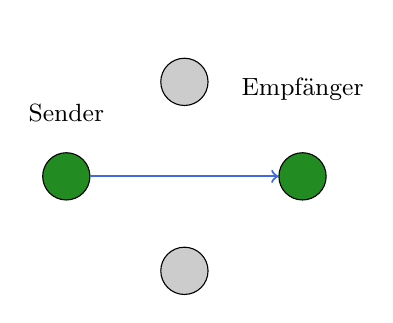
\begin{tikzpicture}[every node/.style={circle,minimum size=6mm,inner sep=0pt}]
                    % Nodes
                    \node[fill=ForestGreen, draw=black] (A) at (0,0) {};
                    \node[fill=ForestGreen, draw=black] (B) at (3,0) {};
                    \node[fill=Gray!40, draw=black] (C) at (1.5,1.2) {};
                    \node[fill=Gray!40, draw=black] (D) at (1.5,-1.2) {};
                    % Labels
                    \node[above,font=\small] at (A.north) {Sender};
                    \node[above,font=\small] at (B.north) {Empfänger};
                    % Arrow
                    \draw[->, thick, RoyalBlue] (A) -- (B);
                \end{tikzpicture}%
            }
            \caption*{\small Unicast: \texttt{1:1}}
        \end{subfigure}\pause\hfill
        \begin{subfigure}[b]{0.26\linewidth}
            \centering
            \resizebox{\linewidth}{!}{%
                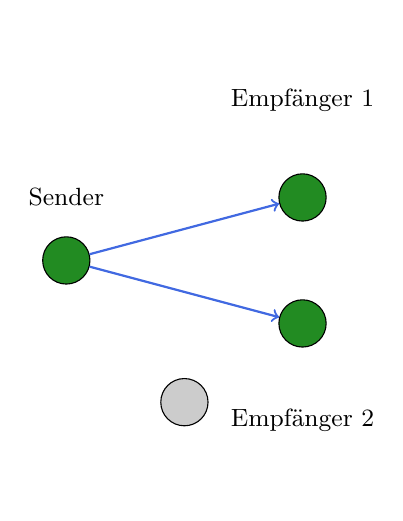
\begin{tikzpicture}[every node/.style={circle,minimum size=6mm,inner sep=0pt}]
                    % Nodes
                    \node[fill=ForestGreen, draw=black] (A) at (0,0) {};
                    \node[fill=ForestGreen, draw=black] (B) at (3,0.8) {};
                    \node[fill=ForestGreen, draw=black] (C) at (3,-0.8) {};
                    \node[fill=Gray!40, draw=black] (D) at (1.5,-1.8) {};
                    % Labels
                    \node[above,font=\small] at (A.north) {Sender};
                    \node[above,font=\small] at (B.north) {Empfänger 1};
                    \node[below,font=\small] at (C.south) {Empfänger 2};
                    % Arrows
                    \draw[->, thick, RoyalBlue] (A) -- (B);
                    \draw[->, thick, RoyalBlue] (A) -- (C);
                \end{tikzpicture}%
            }
            \caption*{\small Multicast: \texttt{1:n}}
        \end{subfigure}\pause\hfill
        \begin{subfigure}[b]{0.26\linewidth}
            \centering
            \resizebox{\linewidth}{!}{%
                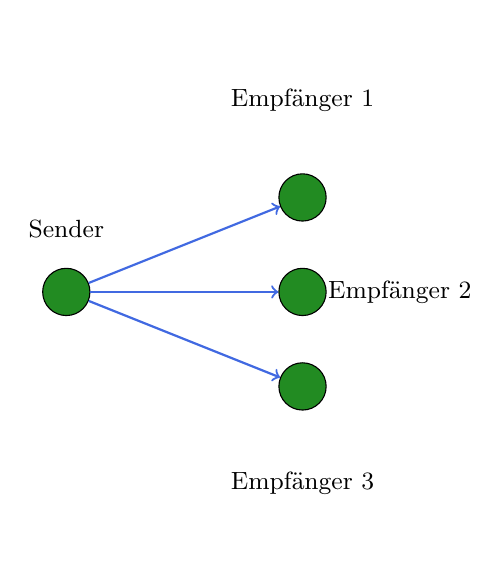
\begin{tikzpicture}[every node/.style={circle,minimum size=6mm,inner sep=0pt}]
                    % Nodes
                    \node[fill=ForestGreen, draw=black] (A) at (0,0) {};
                    \node[fill=ForestGreen, draw=black] (B) at (3,1.2) {};
                    \node[fill=ForestGreen, draw=black] (C) at (3,0) {};
                    \node[fill=ForestGreen, draw=black] (D) at (3,-1.2) {};
                    % Labels
                    \node[above,font=\small] at (A.north) {Sender};
                    \node[above,font=\small] at (B.north) {Empfänger 1};
                    \node[right,font=\small] at (C.east) {Empfänger 2};
                    \node[below,font=\small] at (D.south) {Empfänger 3};
                    % Arrows
                    \draw[->, thick, RoyalBlue] (A) -- (B);
                    \draw[->, thick, RoyalBlue] (A) -- (C);
                    \draw[->, thick, RoyalBlue] (A) -- (D);
                \end{tikzpicture}%
            }
            \caption*{\small Broadcast: \texttt{1:alle}}
        \end{subfigure}
    \end{figure}
\end{frame}

\begin{frame}{Auftrag (\textasciitilde{} 10')}
    \begin{itemize}
        \item \aufgabebox{1.8-1.11}
    \end{itemize}
\end{frame}



